
\chapter{Introduction}


Manipulating the formation of a condensed phase is a critical part of both nature and technology. From molluscs controlling crystal formation~\cite{de-yoreo:03}, to molecular glasses to increasing the solubility of drugs~\cite{hancock:00}, to plastics\tocite, silicon in photovoltaic cells\tocite, and many other materials that we rely on every day. As the devices we use become smaller the need to understand the processes that form them becomes more important. A complete theory of glass formation is still elusive and our ability to control crystal formation is far from what is available to nature. To better understand the formation of the solid phase, we need an understanding of the molecular rearrangements that take place as we move from a molecular liquid, through a supercooled liquid to either a glass or molecular crystal.

\section{Molecular Crystals}

The unit cell is the building block of a crystal. As such it is a useful tool to be able to describe the type of crystal, this is commonly used to describe metal salts. There is the \ce{CsCl} structure, or \ce{NaCl}, Zinc blende and many others. These are used because they are common materials characteristic of their unit cell structure, however the names do not directly inform us of the properties of the underlying unit cell. The simplest descriptor of the unit cell is the shape of the lattice system. There are 7 of these systems~\figref{} representing the different shapes that can be used to pack three dimensional space. Some of these lattice systems can then be combined with a lattice centering, an extra point or points in the lattices. Taking the cubic lattice system, there is the primitive (P) lattice centering where there are only lattice points on the corner of the unit cell which is the lattice of the primitive cubic packing of spheres. The second lattice centering is body centered (I) where there is an additional lattice point in the center of the lattice system resulting in the face centered cubic lattice. There is also the face lattice centering (F) where there is an additional lattice point on each face of the unit cell, for spheres this gives the densest known packing, the face centered cubic packing. The final lattice centering is the base (C) where there is an extra lattice point on one pair of sides. This lattice centering is not present in the cubic lattice system. The combination of these lattice systems and lattice centerings gives the 14 \emph{Bravais lattices}~\figref{}. While extensive, the Bravais lattices are not a complete description of the unit cell, especially in the case of molecules. There are no descriptors of relative orientation of molecules at each of the lattice points, the orientation of each molecule would have to be defined separately. There is a more complete description of the unit cell known as the \emph{Space Group}. The unit cell can be completely recreated from the space group, the unit cell parameters and the position and orientation of a single molecule within the unit cell. Space groups are the combination of a set of symmetry operations and one of the Bravais lattices resulting in 219 space groups, 230 when including chiral copies. There are five symmetry operations that are important to space groups, reflection, rotation, improper rotation (a rotation combined with a mirror plane), screw axis (rotation and translation), and glide plane (reflection and translation)~\figref{}. This complete description of unit cells using space groups allows simple comparisons of crystal structures.

When metallic crystals are grouped into their respective space groups there is a fairly even distribution amongst all the space groups~\figref{}. Do the same with molecular crystals and there is a very different distribution~\figref{}, the P2~\tocheck space group contains a third of all molecular crystals~\tocite and the five most populous space groups contain \SI{75}{\percent} of all molecular crystals. To explain why molecules prefer these space groups over all the others we look to the simpler case of 2D. Using two dimensions has many benefits over a three dimensional system. Computations are far quicker in two dimensions, there are far fewer values to calculate. The visualisation of a two dimensional system on a two dimensional interface such as a computer monitor or a piece of paper does not have to deal with issues such as perspective. This makes visual identification of a pattern or property that incites a 'that's interesting' response far more likely. Another benefit of working in 2D is that there are only 17 \emph{wallpaper groups}~\figref{}, the 2D equivalent of space groups. Wallpaper groups are constructed in the same way as space groups and it is easier to identify the symmetry operations~\figref{}. In a similar manner to 3D we can group all the 2D molecular shapes that have been studied into their wallpaper groups~\figref{}. In this case there are two wallpaper groups that contain the vast majority of molecules, the p2 and the p2gg wallpaper groups. As a general guideline for the packing of 2D molecules without central symmetry \textcite{toquato:12} suggest that the molecules will pair such that the pair will have an inversion center~\figref{}. The only wallpaper groups that support pairs of molecules with this inversion center are the p2 and the p2gg, suggesting that the pairing of molecules has reasonable basis. Now this concept of an inversion center has been identified it can be used as the basis of further investigation in the 3D system.

The way that molecular crystals pack space is an important problem in simulating crystal structures. One of the methods used to find the optimal crystal structure is to model the molecule as an arrangement of hard spheres and find the arrangement of molecules that occupies the largest volume of space~\cite{kitaigorodskii:73}, also known as the \emph{packing fraction}. The simplest example of this is packing spheres, to which Kepler proposed that the hexagonal close packed structure was the most efficient in 1611~\cite{kepler:1611}. The hexagonal close packed structure has the same packing fraction as the face centered cubic structure although being structurally distinct~\figref{}. While these structures have been considered the best possible packing of spheres in space for hundreds of years there has not been a mathematical proof until recently. In 2005 \textcite{hales:05} published a 400 page proof of this problem of which mathematicians were \SI{99}{\percent} certain was correct. Nearly 10 years later \textcite{hales:14} announced the completion of a project to completely satisfy the proof, using computers to check all possible configurations. 

If finding a proof for the simplest of shapes was so difficult, how hard is it going to be to find closest packings for arbitrary shapes. While having a mathematical proof of the closest packed structure is nice, it is not necessary to perform useful chemistry, using the closest known packed structure is a reasonable alternative. Without the requirement for proof of correctness the problem of finding the closest known packing of arbitrary shapes becomes far simpler. The degrees of freedom of the particles can be considered a multidimensional space with the height of that space being the packing fraction~\figref{}, finding the solution is now a case of finding the global minimum of this multidimensional function. Finding the global minimum of a function is a problem that appears in many fields, including computer science. As such there are a number of algorithms that can be used in an attempt to find the global minimum~\tocite. It should be noted that the only method that guarantees finding the global minimum is to evaluate packing fraction at every possible configuration. In 2D, molecules have three degrees of freedom, 2 translational and 1 rotational, if each unit cell has 2 molecules then at minimum there are 6 degrees of freedom. Calculating just 10 points along each degree of freedom, nowhere near enough, requires 1 million calculations of the density, and it scales exponentially with the number of particles. This method very quickly runs into calculations that would take longer than the age of the universe, hence sticking to approximations. Many of these approximations use the concept of simulated annealing~\tocite. This is the process by which the configuration is given an amount of energy to move around the configuration space, moving out of a configuration that has a low packing fraction happens with a high probability, while moving out of a well where the packing fraction is high occurs with low probability. The probability of the configuration moving scales with the energy, as the energy is slowly reduced only the best configurations are sampled. If the energy is reduced slowly enough the global minimum is the final configuration, however there is no way to determine beforehand what slowly enough is. This concept comes from the process of glass formation which will be discussed in~\secref{} and many of the same concepts hold.

\towrite{convex vs concave particles}


\towrite{results of packing stuff}

Along with categorising the crystal structure the unit cell of a crystal structure is also responsible for many of the properties of the resulting material.


\towrite{Properties of solids, magnetic, conductivity, brittleness, piezoelectric}

The periodic and ordered structure that comes from the symmetry of the space group is also responsible for a number of properties of the crystal phase. These include mechanical properties such as hardness~\tocite or brittleness~\tocite, electrical properties\tocite, magnetic properties\tocite, even colour\tocite. For some applications the solid form is necessary however the crystal has unfavourable properties. An example of this is in drug design, a drug administered in tablet form needs to be solid, however it also needs to be soluble\tocite. Or in fiber optics where the fiber needs to be solid but also needs to be flexible\tocite. These applications can benefit from an amorphous solid, also known as a glass.


\section{Molecular Liquids}






\section{Molecular Glasses}

The structure of a glass is indistinguishable from that of a liquid~\figref{}. Despite the liquid like structure the glassy phase is most definitely solid~\tocite, contrary to urban legends~\tocite. Much of the misunderstanding of the glassy phase is related to the lack of a first order phase transition~\tocite. None of the thermodynamic properties change upon transition, instead the \emph{glass transition temperature} (\si{\Tg}) is defined as the temperature at which the viscosity reaches \SI{e13}{\poise}, a somewhat arbitrary value. However as we approach the \si{\Tg} from the liquid there is a dramatic increase in the viscosity~\figref{}, especially for \emph{fragile} liquids.

Glass formers are characterised by their behaviour near \si{\Tg}. Liquids that adhere to a purely Arrhenius temperature dependence are considered \emph{strong} glass formers, the typical example being silica (\ce{SiO2}). Liquids with super-Arrhenius behaviour are considered \emph{fragile}, \emph{o}-terphenyl being the canonical example. A system that displays Arrhenius temperature dependence,
\begin{equation}
    k = A \e^{-E_a/(RT)}
\end{equation}
has an energy barrier that requires an activation energy ($E_a$) to surmount. This activation energy remains constant throughout the temperature range. Fragile liquids however have an activation energy that depends on the temperature\tocite, characterised by large increases in viscosity over a small temperature range as \si{\Tg} is approached. The temperature dependence of the viscosity in fragile liquids indicates that the glass transition temperature is more than just an arbitrary value, rather; the glass transition is an inherent characteristic of a material.

Developing a theoretical understanding of a material requires a model system, something simple enough to model easily, yet close enough to a real world example. A defining feature of fragile glass formers~\tabref{} is the prominence of molecular liquids, making simple molecular liquids a good choice for a model system.


\begin{figure}
    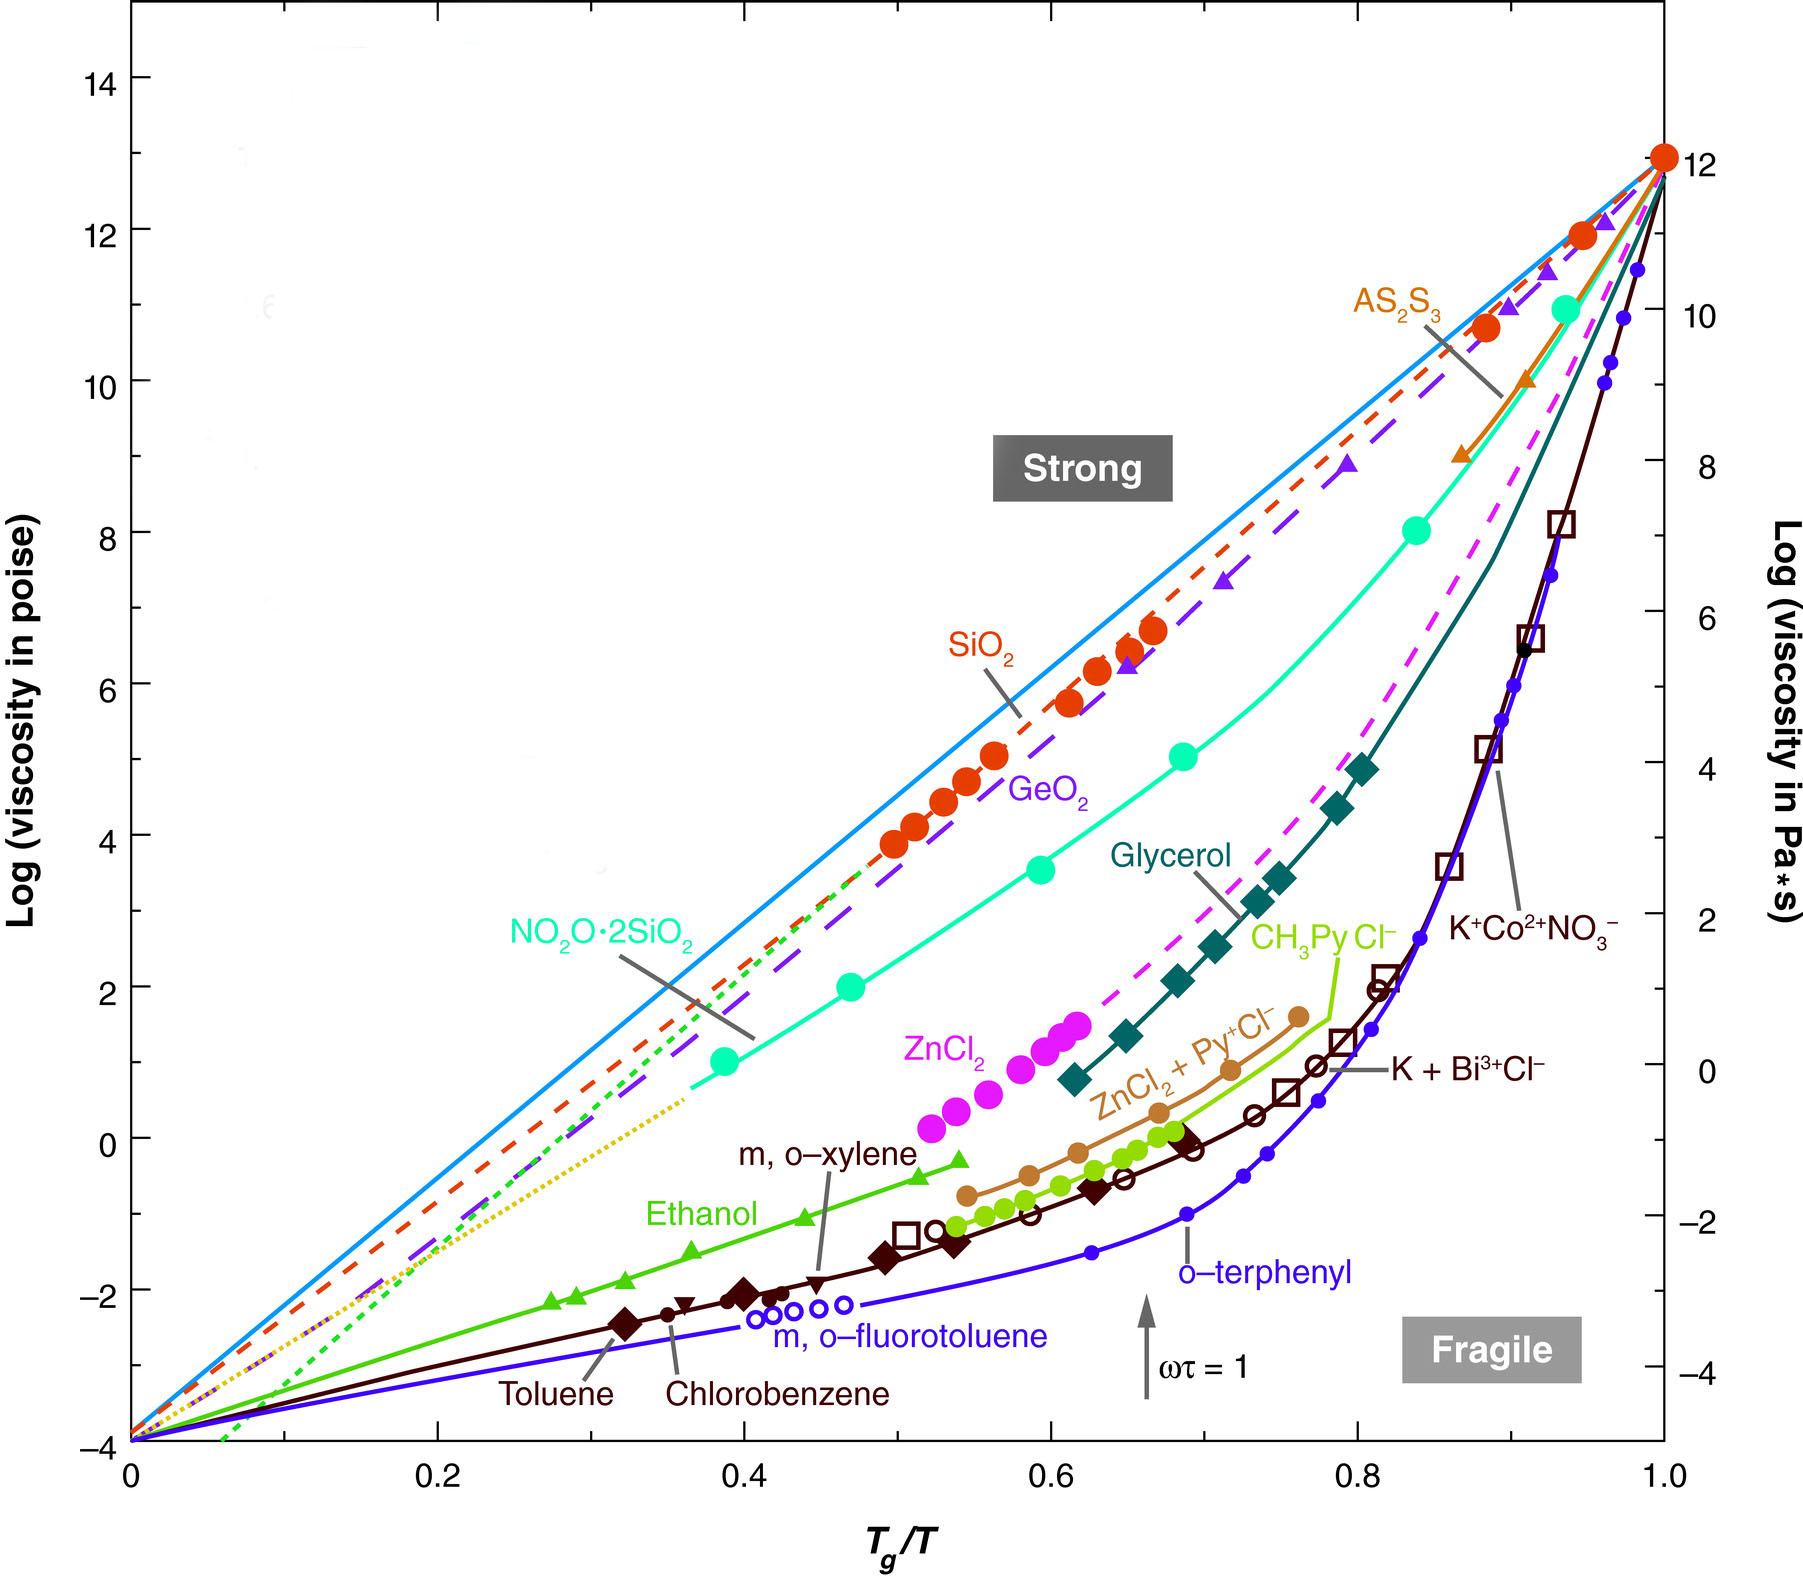
\includegraphics[width=\textwidth]{angell}
    \caption{Angell plot (from \textcite{lubchenko:07}, used with permissioni Annual reviews)}
    \label{fig:entropy}
\end{figure}

\section{Liquids}



\section{Project Goals}

The goal of my project is to explore fundamental features of molecular shape; asymmetry and concavity, influence the properties of the various condensed phases; liquid, crystal, glass and supercooled-liquid. This requires the characterisation of a new set of molecular models for computer simulation. I will be addressing how the molecular orientation and translational motion couple during crystal growth, how the degree of concavity in the molecular shape determines the dynamics of rotations and translations in the low temperature liquid phase and, to find stable structures that determine the properties of crystals and glasses and how these structures are influenced by molecular shape.

